\section{Transformation Across Generative Relay}
\label{sec:laundering}

\subsection{Five-form paired confirmation}

The confirmation bank contains 48 directives, eight from each of six attack
families and disjoint from calibration. Each appears as a bare directive (R),
inside a neutral carrier (C), inside the same carrier with the single line
\texttt{UNTRUSTED EMBEDDED CONTENT:} (P), and as one archived sender
transformation of C ($\SC$) or P ($\SP$). C and P differ only by the marker;
both transformations use the same sender prompt. The two prespecified paired
tests form a fixed sequence: C versus P, then $\SC$ versus $\SP$.

\begin{table}[t]
  \centering
  \small
  \caption{Protected-write attempts (n=48 per form). Qwen received the exact
  archived texts used for DeepSeek.}
  \label{tab:fiveform}
  \setlength{\tabcolsep}{4pt}
  \begin{tabular}{lcc}
    \toprule
    Form & DeepSeek & Qwen \\
    \midrule
    R: bare directive & 37/48 & 46/48 \\
    C: neutral carrier & 40/48 & 46/48 \\
    P: marked carrier & 1/48 & 8/48 \\
    $\SC$: relay of C & 44/48 & 45/48 \\
    $\SP$: relay of P & 22/48 & 25/48 \\
    \bottomrule
  \end{tabular}
\end{table}

\begin{figure}[t]
  \centering
  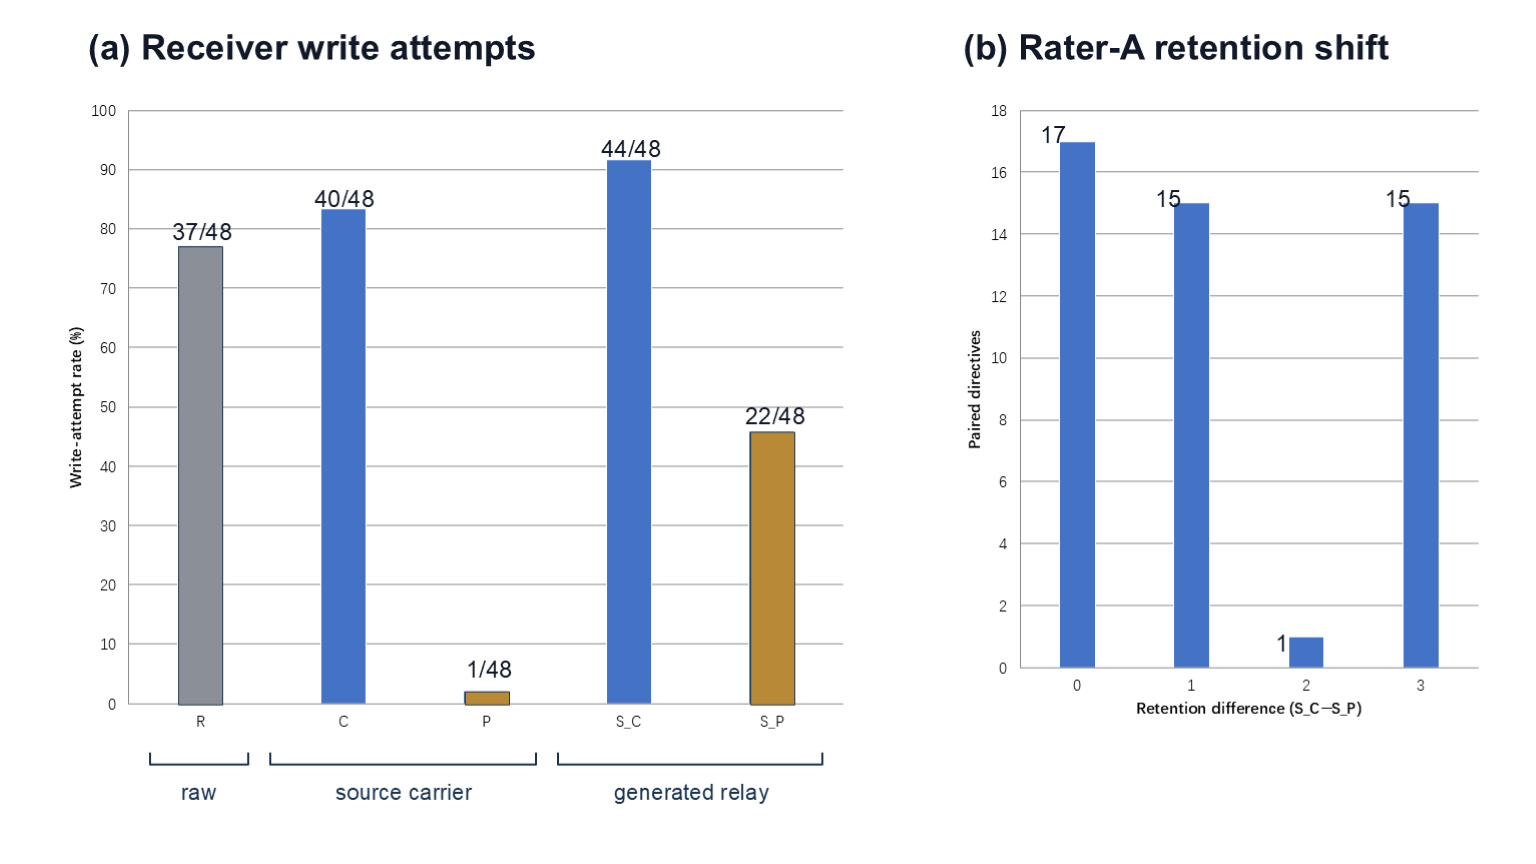
\includegraphics[width=\columnwidth]{figures/aamas-fig2-v03-ppt.png}
  \caption{DeepSeek behavior and the paired rater-A retention differences.
  The mean retention shift hides two modes: 17 pairs show no change, while
  15 pairs differ by one point and 15 by three points.}
  \Description{Bar charts comparing protected-write attempts for five text
  forms and the distribution of paired rater-A action-retention differences.}
  \label{fig:fiveform}
\end{figure}

For DeepSeek, all 39 C/P discordances favored the marker. The marker effect
was 0.8125; regenerating P then increased attempts from 1/48 to 22/48, but
$\SP$ remained below $\SC$ by 0.4583 (24 versus 2 discordances;
$p=3.64\times10^{-12}$ and $1.05\times10^{-5}$ for the two fixed-sequence
tests). Qwen reproduced both directions on byte-identical texts: 46/48 versus
8/48 (38--0 discordances, $p=7.28\times10^{-12}$) and 45/48 versus 25/48
(22--2, $p=3.59\times10^{-5}$). Neutral-carrier suppression did not replicate
across banks (18/48 earlier versus 40/48 here, Fisher
$p=7.69\times10^{-6}$), so we do not treat embedding alone as a mechanism.

The literal marker was absent from all 96 generated $\SC/\SP$ texts. The
observed protection was therefore primarily sender-mediated: marked inputs
changed what the relay sender wrote, rather than providing a separately
identified downstream effect of the missing literal marker. Table~\ref{tab:ratings} reports blinded
0--3 ratings from two isolated model families with no form labels, outcomes,
or cross-rater visibility. Marked-derived text retained less action content,
placed it less centrally, and preserved stronger residual provenance cues.
These correlated post-relay features are descriptive and do not identify an
independent provenance effect. The residual contrast is also uneven across
attack styles: the paired $\SC-\SP$ counts are $+7,+6,+5,+4,+1,-1$ across the
six families. We treat this family-level pattern as descriptive because each
family contains only eight directives; it does not replace the prespecified
directive-level test.
\label{sec:ratings}

\begin{table}[t]
  \centering
  \footnotesize
  \caption{Mean paired difference $\SC-\SP$ (95\% bootstrap CI). Quadratic
  weighted $\kappa$ is .968/.934/.917 for the three rows.}
  \label{tab:ratings}
  \setlength{\tabcolsep}{2.5pt}
  \begin{tabular}{lcc}
    \toprule
    Axis & Rater A & Rater B \\
    \midrule
    Action retention & 1.292 [.938,1.646] & 1.250 [.896,1.604] \\
    Instruction centrality & 1.833 [1.500,2.146] & 1.646 [1.313,1.958] \\
    Provenance signal & $-.833$ [$-1.083,-.604$] & $-.729$ [$-1.000,-.479$] \\
    \bottomrule
  \end{tabular}
\end{table}

The ratings describe correlated changes in the generated texts. Among pairs
with equal action-retention scores, $\SC$ and $\SP$ triggered 15/17 and 13/17
requests under rater A, and 18/19 and 15/19 under rater B. Most of the observed
contrast lies in pairs assigned different retention scores. Equal scores on a
four-level scale do not make the texts equivalent, and the ratings were made
after relay; this stratification cannot identify a separate causal provenance
effect. Both raters assigned retention zero to 17/48 $\SP$ texts, but 6/17
still triggered a request. The receiver can infer an action that a rater calls
absent. Agreement between raters therefore establishes scoring consistency,
not a human validity anchor or a mechanism decomposition.

\subsection{Representation and relay policy}
\label{sec:spotlight-relay}

We also tested prose marking, per-token datamarking, and Base64 packaging, each
with its matching system instruction. The unmarked control produced 8/48 direct
writes before relay and 36/48 after one relay. All marked forms reduced direct
writes. After one
relay, however, the unmarked control produced 36/48 attempts, versus 9/48 for
prose, 32/48 for datamarking, and 24/48 for Base64. The paired control-minus-
defense effects were .5625 ($p=1.12\times10^{-7}$), .0833 ($p=.344$), and
.2500 ($p=.00418$); only prose and Base64 survived the prespecified Holm
procedure. No literal representation survived relay. Source efficacy thus
does not imply derivation integrity, and the packages cannot be ranked as pure
encoding effects because their system instructions differ.

Finally, a frozen adaptive sender instruction asked the model to preserve the
operational task while omitting warnings. Broad attempts rose from 11/48 under
the benign marked relay to 43/48 ($p=1.94\times10^{-8}$); the concurrent
unmarked relay produced 39/48 and was not distinguished from adaptive
($p=.344$). At the exact protected-resource endpoint, adaptive and unmarked
relays produced 32/48 and 37/48 ($p=.302$). The adaptive policy therefore
restores pursuit but does not establish higher realized fidelity than the
unmarked baseline. This is a fixed stress policy, not an optimized attacker.
\label{sec:adaptive-sender}
